% mnras_template.tex 
%
% LaTeX template for creating an MNRAS paper
%
% v3.0 released 14 May 2015
% (version numbers match those of mnras.cls)
%
% Copyright (C) Royal Astronomical Society 2015
% Authors:
% Keith T. Smith (Royal Astronomical Society)

% Change log
%
% v3.0 May 2015
%    Renamed to match the new package name
%    Version number matches mnras.cls
%    A few minor tweaks to wording
% v1.0 September 2013
%    Beta testing only - never publicly released
%    First version: a simple (ish) template for creating an MNRAS paper

%%%%%%%%%%%%%%%%%%%%%%%%%%%%%%%%%%%%%%%%%%%%%%%%%%
\documentclass[fleqn,usenatbib]{mnras}

\usepackage{newtxtext,newtxmath}
\usepackage[T1]{fontenc}
\usepackage{ae,aecompl}


%%%%% AUTHORS - PLACE YOUR OWN PACKAGES HERE %%%%%
\usepackage{graphicx}	% Including figure files
\usepackage{amsmath}	% Advanced maths commands
\usepackage{amssymb}	% Extra maths symbols
\usepackage{subcaption}
\captionsetup{compatibility=false}
\usepackage[capitalise,
            noabbrev]{cleveref} % also needs to be /last-last/
  \creflabelformat{equation}{#2#1#3} % undo parens around equation refs
  \crefname{algorithm}{Function}{Functions}
  \Crefname{algorithm}{Function}{Functions}
  
\usepackage{xcolor}
%%%%%%%%%%%%%%%%%%%%%%%%%%%%%%%%%%%%%%%%%%%%%%%%%%

%%%%% AUTHORS - PLACE YOUR OWN COMMANDS HERE %%%%%

% Please keep new commands to a minimum, and use \newcommand not \def to avoid
% overwriting existing commands. Example:
%\newcommand{\pcm}{\,cm$^{-2}$}	% per cm-squared

%%%%%%%%%%%%%%%%%%%%%%%%%%%%%%%%%%%%%%%%%%%%%%%%%%

%%%%%%%%%%%%%%%%%%% TITLE PAGE %%%%%%%%%%%%%%%%%%%
% Title of the paper, and the short title which is used in the headers.
% Keep the title short and informative.
\title[Phase Lags for OH/IR stars]{
Phase lag determination for OH/IR stars from the Hartebeesthoek OH monitoring programme
}

% The list of authors, and the short list which is used in the headers.
% If you need two or more lines of authors, add an extra line using \newauthor
\author[M. E. West et al.]
{M. E. West$^{1,2}$\thanks{E-mail: marion@hartrao.ac.za},
R. van Rooyen$^{2}$,
\\
% List of institutions
$^{1}$Hartebeesthoek Radio Astronomy Observatory,
PO Box 443, Krugersdorp, 1740, South Africa \\
$^{2}$South African Radio Astronomy Observatory,
2 Fir Street, Black River Park, Observatory, Cape Town, 7925
}

% These dates will be filled out by the publisher
\date{Accepted XXX. Received YYY; in original form ZZZ}

% Enter the current year, for the copyright statements etc.
\pubyear{202?}

% Don't change these lines
\begin{document}
\label{firstpage}
\pagerange{\pageref{firstpage}--\pageref{lastpage}}
\maketitle

% Abstract of the paper
\begin{abstract}
{\color {red}
\textbf{Marion to add abstract here...}
}
\end{abstract}

% Select between one and six entries from the list of approved keywords.
% Don't make up new ones.
\begin{keywords}
masers --
stars: OH/IR --
stars: AGB --
methods: data analysis --
methods: periodogram
\end{keywords}
%%%%%%%%%%%%%%%%%%%%%%%%%%%%%%%%%%%%%%%%%%%%%%%%%%

%%%%%%%%%%%%%%%%% BODY OF PAPER %%%%%%%%%%%%%%%%%%
\section{Introduction}
OH/IR stars are late-type stars in the AGB phase of stellar evolution, undergoing substantial mass loss and enshrouded in a thick, expanding shell of dust
\citep[][review]{WilBar68,RJC89}.
The central star heats the dust which re-radiates in the IR.
OH is formed in the outer regions of the dust shell through photo-dissociation of water molecules by UV light.
The thickness of the dust shell, together with the expansion, results in long column densities of OH molecules travelling at velocities with a narrow range of dispersion.
This velocity coherence amongst the OH molecules allows for masing in the dust shell pumped by far-IR photons.
The masers have a characteristic double-peaked profile at 1612 MHz
\citep[][review]{WilBar72,RJC89}
with the most intense radiation arising from the near- and far-sides of the dust shell along the line of sight to the observer.

The central star pulsates resulting in variable heating of the dust and hence IR variations which follow the fluctuations of the central star.
OH maser variations follow the IR variations.
Monitoring the fluctuations in the OH maser radiation allows the phase lag between radiation coming from the front and back of the dust shell to be measured.
This yields the physical size of the OH shell around the star.
The angular diameter of the shell can be measured using interferometry and by combining the two measurements an independent estimate of the distance to the star can be obtained.
The distance measurement is only valid if the OH masing shell obeys the thin shell model
\citep[][review]{ReidMMJS77,RJC89},
ie. it is thin relative to the size of the dust shell and is spherically symmetric.

Determining phase lags from real data appears simple in principle but is non-trivial in practice
Several papers addressing the problem of determining phase lags from lensed quasars highlight some of the difficulties encountered in finding suitable methods
\citep[eg.][]{PhLGil-M02,PhLOscoz01,PhLPelt96,PhLPress92,EK88}.
Standard analytical techniques are appropriate where underlying functions are continuous, stationary, stochastic and regularly sampled
\citep{Welsh99,EK88}.
Real astronomical data rarely fit these criteria.
The \mbox{HartRAO} OH time series, as is generally the case, are continuous and stochastic, but are neither stationary nor regularly sampled.

To determine the phase lag between radiation from the front and back of the OH shell an estimate of the frequency and period of each signals must be obtained.
The HartRAO monitoring data are frequently sampled, making the data well suited for periodogram calculation using the Lomb-Scargle periodogram.
The Lomb-Scargle periodogram is a well-known algorithm for detecting and characterising periodic signals in unevenly sampled data
\citep{2018ApJS..236...16V}.

The HartRAO OH-IR monitoring data will now be publicly available.
The aim of this work is to present a sample of the monitoring data, along with processing methods for phase-lag calculation.

The observational data used in the analysis is described in \cref{sec:observations}.
Data analysis methods are explained in \cref{sec:analysis}.
We present our results on a few selected sources in \cref{sec:results}.
{\color {red}
TBD: \cref{sec:irdata} IR data
}
Lastly, \cref{sec:discussion} present a short discussion of our results.

\section{Observations}
\label{sec:observations}

A set of 20 OH/IR stars was selected for monitoring in the ground state OH lines using the 26--m telescope at Hartebeesthoek
\citep{West98}.
They were monitored from late 1985 until early 1996.
Initially observations were made every two weeks, but the rapid increases in brightness for some of the sources were found to be undersampled and as a result the observing frequency was increased to once a week in mid 1993.
GLONASS interference affected the data
\citep{ComWestGay94}
and this eventually led to the termination of the programme.

The HartRAO antenna had an aperture efficiency of 0.51 when the subreflector was tilted for observing with the off-axis 18cm feed horn.
The beamwidth was $0.5^\circ$ and the pointing accuracy was $30''$.
The spectrometer accepted only one polarization, and left circular
polarization was normally used.  The zenith system temperature was typically 40--50 K.
A correlator bandwidth of 0.64--MHz, covered by 256 channels, provided a velocity resolution of 0.45 km s$^{-1}$.
Most sources were observed at 1612--MHz, although some were also observed at 1665-- and 1667--MHz.
The {\em rms\/} noise on a single fifteen minute spectrum was 0.6 Jy.
Standard continuum sources
\citep{Ott94}
and the 1667--MHz OH absorption towards W12 were used for calibration.

Baseline curvature in the spectra was removed by subtracting low-order polynomials fitted to signal-free segments.
Atmospheric absorption was corrected using a formula obtained from the Jodrell Bank Observatory.
Data affected by rain and the proximity of the Sun were discarded.
After correction, spectra taken in any given 24--hour period were averaged.
Time series were created for all channels with a useful signal to noise ratio.

Interference from GLONASS satellites increased the noise level in the spectra, suppressed the maser lines, affected the system temperature calibration and introduced excessive curvature into the spectrum baselines
\citep{ComWestGay94}.
Manual correction of GLONASS interference
\citep{West98}
was the method of choice for the sources presented in the paper.
The maximum and minimum light curves of the sources shown in \cref{sec:results} uses this cleaned data.
{\color{red}
\textbf{Marion: add a short summary of the evaluation methods applied to manually clean the data?}

Please reference your table of sources here \cref{app:sources}
}

This is however a very time consuming process.
Iterative outlier rejection schemes that systematically smooths and detrends the time series data of an individual channel can be employed to recursively identify and remove outliers greater than 3$\sigma$.
Such an automated outlier rejection scheme is suggested in \cref{app:cleaning}.
The algorithm implementation was tested against the manually corrected data of the sources.
Reducing the need for manual removal to a minimal intervention.

\section{Analysis}
\label{sec:analysis}

Time series analysis of astronomy data is slightly more challenging because the data tends to be stochastic, non-stationary and irregularly sampled.
Making it an uncomfortable fit for standard signal processing methods.
% Consequently, this generally requires some form of up-sampling through interpolation methods, as well as data conditioning such as normalisation.
To determine the phase lag and coherency of the HartRAO OH monitoring data, appropriate methods are selected to deal with the idiosyncrasies of the observed data.

The HartRAO OH time series data monitored pulsed radiation from OH/IR stars over a multi-year campaign, providing good quality, frequently sampled observational data.
The ligth curves contains multiple cycles of periodic signals, and are well suited for analysis using the Lomb-Scargle periodogram
\citep{2018ApJS..236...16V}.

In order to robustify the numerical calculations, some pre-processing of the data was done before analysis.
This was limited to the manual removal of excessive outlier data points, commonly associated with GLONASS interference, as discussed in \cref{sec:observations}.
Given the high sample rate and length of the HartRAO time series data, excessive smoothing is not required and removal of extreme outliers is generally sufficient.
More automated cleaning can also be accomplished using signal processing algorithms such as the Savitzky Golay smoothing filter
\citep{1964AnaCh..36.1627S}.
A detailed discussion of this scheme is provided in \cref{app:cleaning} applied to the maximum light curve for IK Tau (\cref{fig:iktaublueclean}).
Since the HartRAO OH maser monitoring program spanned several years, some time series data may require removing long term trends introducing a bias over time.
This is easily achieved by fitting and subtracting a low order polynomial to the time series.

To calculate the phase difference (lag) between two signals, an estimate of the frequency (or period) of the signals is obtained.
The Lomb-Scargle periodogram is widely used in the analysis of the light curves of variable stars
\citep{1990ApJ...348..700K}.
In essence, the ``fast Lomb-Scargle algorithm'' computes a Fourier-like power spectrum based on the NFFT algorithm that provides an estimate of the period of oscillation for the variable time series
\citep{1989ApJ...338..277P,2018ApJS..236...16V}.
Only a few oscillations are required for computation and the computational effort is similar.
The Lomb-Scargle periodogram, selects a suitable frequency grid automatically based on the input data.
It should be noted that sometimes irregularly-sampled data can be severely undersampled, requiring the user to specify a higher Nyquist frequency when computing the periodogram
\citep{2006MNRAS.371.1390K}.

Once a period is obtained, the time series can be folded by plotting the periodogram as a function of phase rather than time.
This superimposes the periodic cycles over each other, clearly showing the shape of a cycle.
The HartRAO OH monitoring data is very well sampled and do not require folding to extract the shape of the periodic cycles.
% It does show the distribution of frequency and amplitude of the cycles over the multi-year monitoring period.
\section{Results}
\label{sec:results}
We are presenting the results of our analysis on a few selected sources from the OH monitoring data presented in \cref{sec:observations}.
Full spectrum emission between the prominent red and blue peaks were not detectable for all targets, but the spectral profile of all targets shows the canonical `U' shape of a spherical-shell OH/IR star.
The OH monitoring data covers a 7 year period with all targets well sampled over the latter 5 years of observation.
Each time series contained about 260 samples after outlier removal, providing $\sim170$ samples per cycle.
Before period and phase lag calculations all long term trends were removed from the data.

{\color{red}
Five data sets were selected for discussion, namely:
IK Tau a strong Mira variable with a period of approximately 15 months, which shows an interesting double feature red-shifted peaks;
{\color{red}
V Mic: a weaker OH-IR source ...;
}
{\color{red}
WX Psc, OH1.1--0.8 and OH357.1--1.3 
}

\textbf{Marion you need to provide a little more description of each source and why it was included in the discussions of this paper.
What makes them interesting from an observational perspective.}
}


\subsection*{IK Tau}
IK Tau is a Mira variable with an observed period of 470 days listed in the General Catalogue of Variable Stars
\citep{2017ARep...61...80S}.
Under the assumption that the OH masers are pumped during the mass loss phase of the star, we expect period calculation for the blue and red channels from the OH monitoring data to have similar periods.
For the IK Tau OH monitoring observations we identify the blue peak at around 17.4 km/s, but also see two very distinct peaks at the far side maser region (\cref{fig:iktauspectrum}).
The velocity for the nearest red peak is approximately 46.9 km/s, while the velocity of the second (farthest) peak is 50.6 km/s.
{\color {red}
\textbf{Discuss/speculate about the double peaks in the red-shifted features.}
}

The blue peak show a slow but systematic increase in the baseline, \cref{fig:iktau}, that can be best fitted with a low gradient linear polynomial.
Comparing the time series data for the two red peaks we see similar behaviour during the initial cycles with diverging behaviour only becoming apparent in the last two cycles.
Here the baseline of the farthest peak increase drastically compared to the steady increase of previous cycles with the amplitude of the last cycle also increasing significant to be comparable to the the amplitude of the blue peak (\cref{fig:iktautimeseries1}).
Since this is the last of the monitoring data, it is impossible to speculate whether this is a persistent trend or a flare event.
In comparison, the amplitude and baseline of the first red peak remain unchanged, continuing the same trend over the entire monitoring period.
The time series data for this peak shows the same slow linear increase in the baseline as the blue peak, with no visual increase in amplitude (\cref{fig:iktautimeseries0}).

IK Tau is a strong source with five (5) complete and well sampled cycles for period calculation.
We calculated the period for all three peaks, as well as the phase lag between each of the red peaks and the single blue peak.
The Lomb-Scargle periodogram was used to determine the dominant period (in days) per channel.
Given the assumption of the OH masers on the near and far side of a spherical dust shell and experiencing the same pumping mechanism, we would expect the period of the channels to be reasonably similar.
Indeed, all channels show a period of 472.58 days (\cref{fig:iktauperiod}), which is in good agreement with the observed Mira period.
Standard cross-correlation methods were then applied to obtain the phase difference between the time series data of the red and blue peaks, with the 
red channel at 47 km/s and the blue channel showing close correlation between time series signals.
Correlation show the red channel lagging the blue channel by less than a day (0.245 days).
The farthest red channel was found to lag behind the blue channel much more, by around 7.261 days.


\subsection*{V Mic}
Similar to IK Tau, V Mic is a Mira variable with an observed period of 381.15 days from the General Catalogue of Variable Stars
\citep{2017ARep...61...80S}.
However, V Mic is a weak OH-IR source for which the blue and red channels were selected as shown in the spectrum plot \cref{fig:vmicspectrum}.
Time series data for the channels show a flat trend over time and no visible change in amplitude for either of the channels.
The red channel is however, significantly dimmer than the blue channel and the data for the red channel is much noisier as a result.
The time series of V Mic also has five (5) complete cycles and are well sampled over the latter four (4) or these cycles (\cref{fig:vmictimeseries}).

Being a weak source also makes period and phase difference calculation more uncertain.
Period calculation gave period of 378.45 days and 391.28 days for the blue and red channels respectively (\cref{fig:vmicperiod}).
An average period of 384.86 days was thus assumed, which is in agreement with the observed stellar period.
This average period provides a phase difference of 4.9 days between the red and blue channels.
{\color {red}
Marion to add xref of Martin Shepard's thesis -- delay noted and please add reference
}


\subsection*{WX Psc}
{\color{gray}
WX Psc is a weaker source with a period of two years and seven cycles of data, shown in \cref{fig:wxpsctimeseries}.
By contrast with OH357.1--1.3, WX Psc has narrow peaks with no noticeable emission in between (\cref{fig:wxpscspectrum}).
The brightest blue-- and red--shifted peaks are represented by channels 2 and 3 and channels 11 and 12 respectively.
There were 330 samples across the whole time series.
For cycles 1 -- 4.5, observed at two-week intervals, there were typically $\sim45$ samples per cycle, albeit with significant gaps in cycles 1 and 2.
The remaining one and a half cycles had double the number of samples per cycle.
}


\subsection*{OH357.3--1.3}
OH357.1–1.3 is a strong source but being slow varying means that over the multi-year OH monitoring program only one complete cycle was observed.
Clear peaks are visible in the spectral profile and emission is detectable  at all points between the two peaks (\cref{fig:oh357spectrum}).
The time series of the associated brightest blue- and red-shifted peaks clearly displays the typical nature of light curves with asymmetry between the rise and decay periods of the light curves (\cref{fig:oh357timeseries}).
Other than for IK Tau and V Mic, the red channel are comparable in amplitude rather than weaker than the blue channel.
It also shows a clear increase in amplitude over the second peak in the time series data and the peak profile appears sharper than the first peak period.
The two peaks in the time series data are more similar.
Visually there seem to be some delay between the 2 signals, but given the asymmetry in the signal and only a single observed period the signals will not fold well, making period calculation using numerical methods a little more challenging.
Numerical and statistical methods require at least a few cycles in the data in order to compute a wide enough range for the frequency grids
\citep{2018ApJS..236...16V}.
For this source, period estimation was thus done manually, by selecting the initial period as the time between the two peaks for each channel, and then refining the period by folding the data around the initial period until a reasonable folded profile was obtained (\cref{fig:oh357period}).
An approximate period of 2141.4213 days was identified as the best fit.
Using this period for cross correlation calculations provided a phase shift of 48.9034 days between the maximum and minimum light curves for OH357.1–1.3.
{\color {red}
Marion xref with lag determined by thesis
}


\subsection*{OH1.1--0.8}

{\color {red}
\section{IR data}
\label{sec:irdata}
}
\section{Discussion}
\label{sec:discussion}

{\color {red}

\textbf{Marion can you please help with reconciling this discussion with the one in the older article, as well as comparison of results as indicated}

Marion: what does the phase differences tell us and how can they be used.


\textbf{Ruby need to discuss data for the sources presented, as well as all the data analysis techniques discussed can be found}
}
Example files and processing scripts used to generate the results presented in this article can be found on GitHub (\mbox{\url{https://github.com/rubyvanrooyen/HartRAO_OH-IR_stars}}).

\section*{Acknowledgements}

The authors thank staff at HartRAO who
helped with running the observations.

%%%%%%%%%%%%%%%%%%%% REFERENCES %%%%%%%%%%%%%%%%%%
\bibliographystyle{mnras}
\bibliography{mn-jour,refs-adsabs}
%%%%%%%%%%%%%%%%%%%%%%%%%%%%%%%%%%%%%%%%%%%%%%%%%%

% IK Tau
\begin{figure*}
\centering
  \begin{subfigure}{\hsize}
    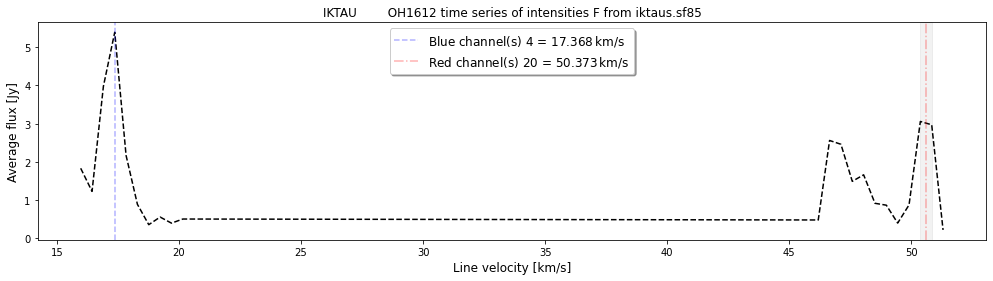
\includegraphics[width=0.95\hsize]{images/IKTau_avg_spectrum.png}
    \caption{\label{fig:iktauspectrum}Spectral profile show double narrow red peaks with no noticeable emission in between the blue peak and the red peaks. For flattened peak structures, such as for the red peaks, an average of the channels over that flat peak was used, rather than a single channel.}
  \end{subfigure}%
  \\
  \begin{subfigure}{\hsize}
    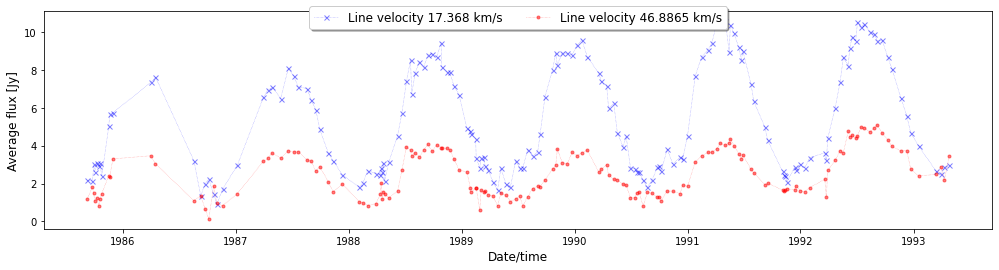
\includegraphics[width=0.95\hsize]{images/IKTau_ts_blue4_red12.png}
    \caption{\label{fig:iktautimeseries0}Time series of red peak show significantly weaker signal than blue peak. Both blue and red time series show similar behaviour over the monitoring period with a slow linear increase in baseline (most noticeable toward the end) and consistent amplitude over time.}
  \end{subfigure}%
  \\
  \begin{subfigure}{\hsize}
    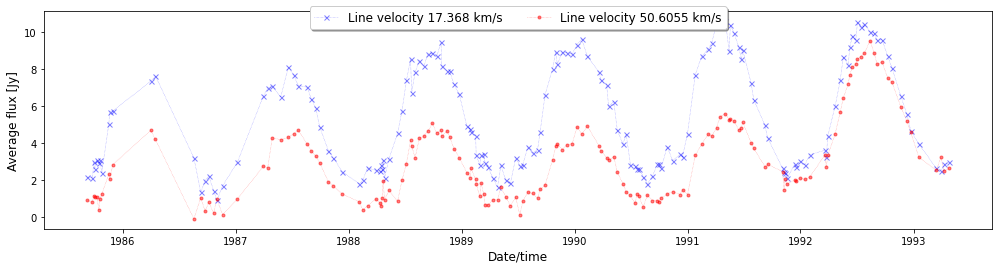
\includegraphics[width=0.95\hsize]{images/IKTau_ts_blue4_red20.png}
    \caption{\label{fig:iktautimeseries1}The time series data for this peak show significant changes during the last monitoring cycle with not only a strong increase in baseline, but also a significant increase in strength with the amplitude of the last cycle comparable to the amplitude of the stronger blue line.}
  \end{subfigure}%
\caption{\label{fig:iktau}The 1612 MHz OH spectrum of IK Tau at maximum and minimum light.}
\end{figure*}

\begin{figure*}
\centering
  \begin{subfigure}{0.33\hsize}
    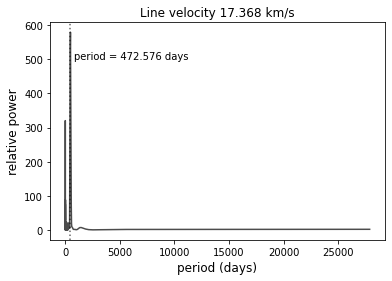
\includegraphics[width=0.99\hsize]{images/IKTau_blue_17.368_periodogram.png}
  \end{subfigure}%
  \hfill
  \begin{subfigure}{0.33\hsize}
     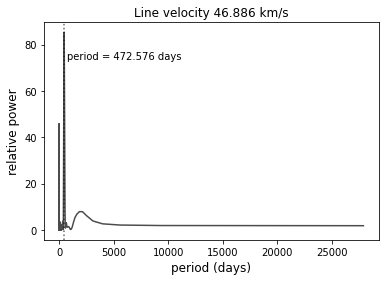
\includegraphics[width=0.99\hsize]{images/IKTau_red_46.886_periodogram.png}
  \end{subfigure}%
  \hfill
  \begin{subfigure}{0.33\hsize}
    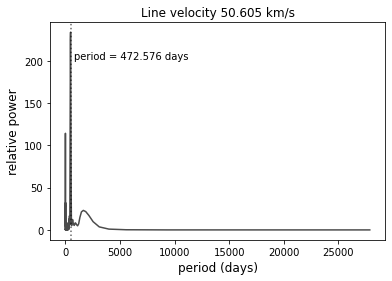
\includegraphics[width=0.99\hsize]{images/IKTau_red_50.605_periodogram.png}
  \end{subfigure}%
\caption{\label{fig:iktauperiod}Lomb-Scargle periodogram calculations for IK Tau blue and red channel time series data give average period of 472.576 days.}
\end{figure*}


% VMic
\begin{figure*}
\centering
  \begin{subfigure}{\hsize}
    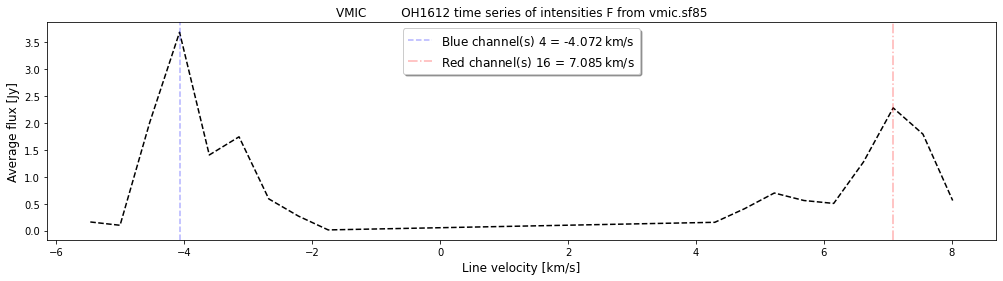
\includegraphics[width=0.95\hsize]{images/VMic_avg_spectrum.png}
    \caption{\label{fig:vmicspectrum}Identification of the the blue and red channels are not well defined narrow peaks, so simple maximum value evaluation was used for channel selection.}
  \end{subfigure}%
  \\
  \begin{subfigure}{\hsize}
    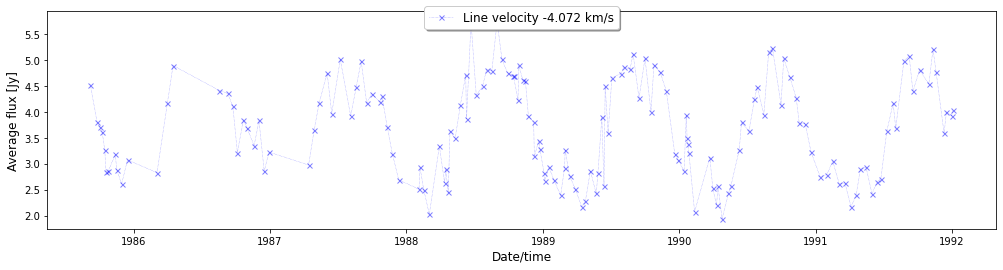
\includegraphics[width=0.95\hsize]{images/VMic_ts_blue4.png}
    \caption{\label{fig:vmictimeseries}Since V Mic is such a weak source, it is difficult to distinguish the time series data for the blue (-4.072 km/s) and red (7.085 km/s) channels if plotted in overlay. For this reason only the the time series for the stronger blue channel is displayed.}
  \end{subfigure}%
\caption{\label{fig:vmic}The 1612 MHz OH spectrum of VMic at maximum and minimum light.}
\end{figure*}

\begin{figure*}
\centering
  \begin{subfigure}{0.5\hsize}
    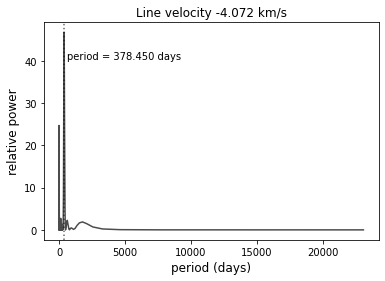
\includegraphics[width=0.99\hsize]{images/VMic_blue_-4.072_periodogram.png}
  \end{subfigure}%
  \hfill
  \begin{subfigure}{0.5\hsize}
    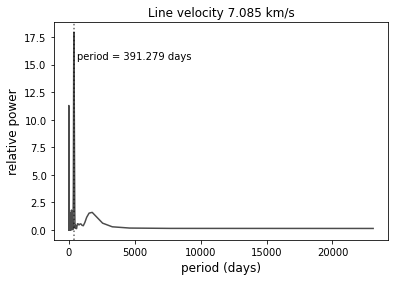
\includegraphics[width=0.99\hsize]{images/VMic_red_7.085_periodogram.png}
  \end{subfigure}%
\caption{\label{fig:vmicperiod}Lomb-Scargle periodogram calculations for V Mic blue and red channel time series data give differing period for the blue and red channels. This difference is expected since the source is weak, but the average period of 384.86 days gives a reasonably good fit to the data and agrees well with the stellar period.}
\end{figure*}

\begin{figure*}
\centering
  \begin{subfigure}{\hsize}
%    \includegraphics[width=0.95\hsize]{images/}
    \caption{Spectral profile show narrow peaks with no noticeable emission in between.}
    \label{fig:wxpscspectrum}
  \end{subfigure}%
  \\
  \begin{subfigure}{\hsize}
%    \includegraphics[width=0.95\hsize]{images/}
    \caption{Light curves of brightest peaks are averaged power of neighbouring blue- and red-shifted peaks.}
    \label{fig:wxpsctimeseries}
  \end{subfigure}%
\caption{\label{fig:wxpsc}The 1612 MHz OH spectrum and light curve of WX Psc at maximum and minimum light.}
\end{figure*}


\begin{figure*}
\centering
  \begin{subfigure}{\hsize}
    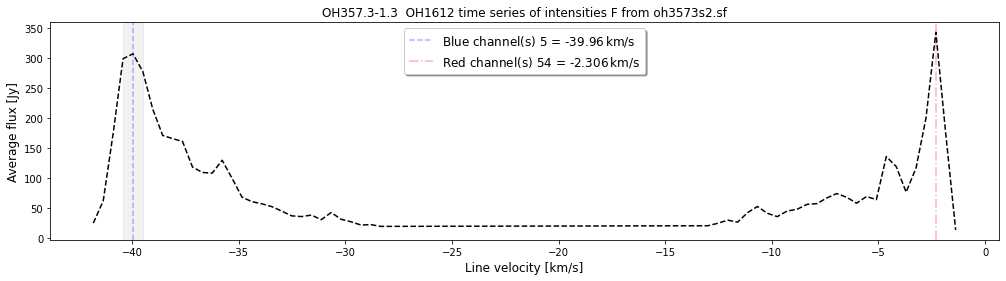
\includegraphics[width=0.95\hsize]{images/OH357_avg_spectrum.png}
    \caption{\label{fig:oh357spectrum}Spectral profile showing the canonical `U' shape of a spherical dust shell around OH/IR stars. The spectrum show clear blue and red peaks, with the blue peak taken to be the average of the 3 channels at maximum.}
  \end{subfigure}%
  \\
  \begin{subfigure}{\hsize}
    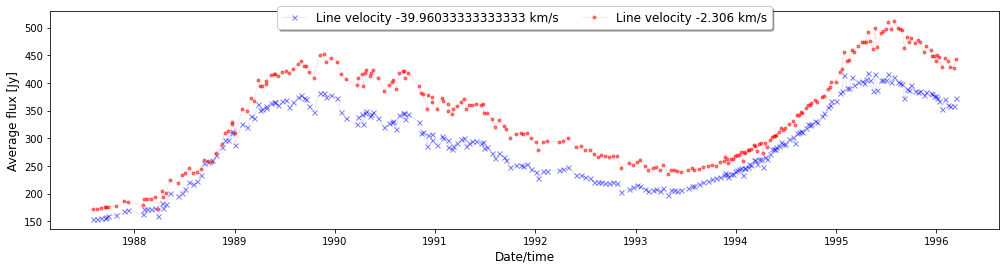
\includegraphics[width=0.95\hsize]{images/OH357_ts_blue5_red54.png}
    \caption{\label{fig:oh357timeseries}Time series of brightest blue- and red-shifted peaks show single period over 6 years. The second peak of the red channel sow a mark increase in amplitude and asymmetry in shape. Visually there seem to be some delay between the 2 signals.}    
  \end{subfigure}%
\caption{\label{fig:oh357}The 1612 MHz OH spectrum and light curve of OH357.1--1.3 at maximum and minimum light.}
\end{figure*}

\begin{figure*}
\centering
  \begin{subfigure}{\hsize}
    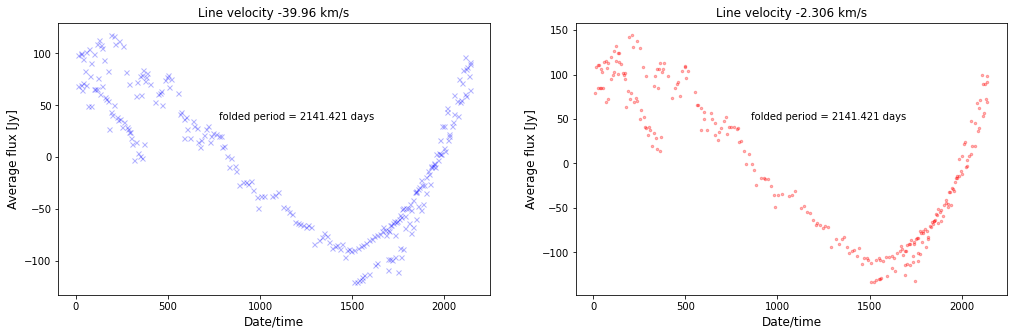
\includegraphics[width=0.99\hsize]{images/OH357_ts_blue5_red54_detrended_folded.png}
  \end{subfigure}%
\caption{\label{fig:oh357period}Folded time series for manually established best fit period of 2141.421 days for both blue and red channels.}
\end{figure*}


\begin{figure*}
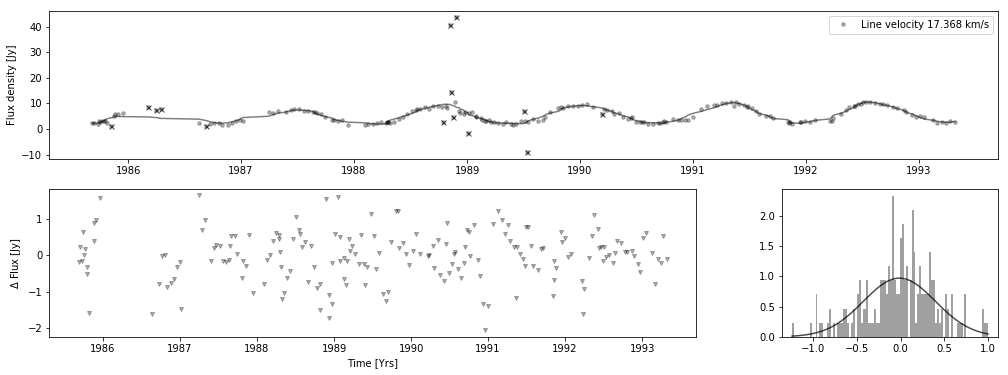
\includegraphics[width=\hsize, clip,angle=0]{images/iktausRAW_blue_channels_cleaned.png}
\caption{\label{fig:iktaublueclean}The dots in the top graph show the cleaned time series data for IK Tau blue channel. While the crosses indicates the discarded outliers. To evaluate how well the smoothed curve fit the data the residual is shown as triangles in the lower left plot. The histogram of the residual, lower right plot, is used for visual evaluation with the process continued until this distribution indicates a reasonable noise like character to the residual.}
\end{figure*}


%%%%%%%%%%%%%%%%% APPENDICES %%%%%%%%%%%%%%%%%%%%%

\appendix
\section{Tables of sources}
\label{app:sources}
{\color {red}
\textbf{Marion add your tables here please}
}


\section{Automated cleaning of spectra}
\label{app:cleaning}

Automated detection and removal of data points outside a 3 sigma deviation from the mean will assist manual removal of outliers in the selected channels.
The identification of these outliers requires some form of smoothing, which can be accomplished using robust signal processing algorithms such as the Savitzky Golay smoothing filter
\citep{1964AnaCh..36.1627S}.
In an iterative process a curve is fitted to the data and subtracted from the original to obtain a residual.
This residual is used to identify and remove outliers, after which the cleaned data is used to repeat the process.
A conservative approach is taken when implementing this automatic cleaning of the data to void over-cleaning.
Opting for manual intervention to remove the remaining few outliers after the automated process had finished.
The results from such an automated run applied to the blue channel of IK Tau is shown in \cref{fig:iktaublueclean}.

Since we chose conservative thresholds and smoothing windows, we found that we generally needed to repeat the iterative auto-cleaning process at least twice for signals that have sections with large scatter.
Especially if those outlier points were distributed over a range of deviations from the mean, such as can be seen in our example IK Tau data series (\cref{fig:iktaublueclean}) around 1989 observation period.
Visualisation of the cleaned output data after each cleaning run was used to verify the success of the cleaning step.

Even though we used the cleaned data for the analysis, we tended to detrend the data before calculation.
The HartRAO OH maser monitoring program spanned several years.
This removal of long term trends over the years that the OH monitoring program was observed tend to help the numerical methods that will apply some form of normalisation, such as subtracting the mean, to the data.
Subtracting low order polynomial removes these long term trends in the data, and notebooks showing this process can be found on GitHub (\mbox{\url{https://github.com/rubyvanrooyen/HartRAO_OH-IR_stars}}).


%%%%%%%%%%%%%%%%%%%%%%%%%%%%%%%%%%%%%%%%%%%%%%%%%%


% Don't change these lines
\bsp	% typesetting comment
\label{lastpage}
\end{document}

% End of mnras_template.tex